\documentclass[uplatex, titlepage, dvipdfmx, 12pt, a4paper]{jsreport}
\usepackage{geometry}                		% See geometry.pdf to learn the layout options. There are lots.
\geometry{margin=2.5cm}                   		% ... or a4paper or a5paper or ... 
%\geometry{landscape}                		% Activate for rotated page geometry
\usepackage[parfill]{parskip}    		% Activate to begin paragraphs with an empty line rather than an indent
\usepackage[dvipdfmx]{graphicx}				% Use pdf, png, jpg, or eps§ with pdflatex; use eps in DVI mode		
\usepackage{amssymb}
\setcounter{tocdepth}{3}

\title{ \huge 卒業論文\\ \Huge リングイメージ型検出器(RICH)\\の性能評価}
\author{ \LARGE 戸田 匡哉 \and \LARGE 徳田 恵}
\date{\Large \today}							

\begin{document}
\maketitle
\begin{abstract}
 我々は J-PARCハドロン実験施設の高運動量ビームラインにおいてチャームバリオン分光実験 (J-PARC-E50) を計画している。実験では運動量20 GeV/{\sl c} のビーム粒子と標的との反応で生成する 2$\sim$16 GeV/{\sl c}の高運動量散乱粒子の識別を行う必要がある。この広い運動量領域において粒子識別を行うためにリングイメージチェレンコフ検出器を開発している。\\
 粒子識別性能に関わる角度分解能のうち、収差等の内訳を調べるため、テスト機を用いてSPring-8 のLEPSビームラインにおいてテスト実験を行った。光センサーとしてMPPCアレイを使用し、同時にMPPCの暗電流による角度分解能への影響や電圧依存性を調査した。MPPCアレイは8$\times$8の64セグメントで、各セグメントの大きさが3mm$\times$3mmのものを用いた。実験では空気を輻射体とし、0.95 GeV/{\sl c}の電子・陽電子からのチェレンコフ光を球面鏡によってMPPCアレイ上に結像させた。また、MPPCの動作電圧を0.5Vずつ54.0V-57.5Vの間で変化させ、取得したTDCデータからリングイメージを測定した。\\
 得られたリングイメージからリング中心を決定しイベント毎にチェレンコフ角を計算、角度分解能のhit数依存性から角度分解能をセグメントサイズによる位置分解能$\Delta\theta_{seg}$と、収差などによる分解能$\Delta\theta_{other}$に分けた。セグメントサイズによる位置分解能は用いたMPPCの1セグメントの大きさと球面鏡の焦点距離から計算によって求められ、$\Delta\theta_{seg}=2.80$ mradとなる。収差などによる分解能は、角度分解能のhit数依存性のグラフからフィッティングから見積もり、$\Delta\theta_{other}=3.88 \pm 0.02$ mradとなった。ここから焦点面と検出面の位置のずれや、入射粒子の角度分解能、色収差などに細分し、残ったものを暗電流の影響とした。\\
 また各動作電圧でのイベントごとのhit数から、hit数の電圧依存性とシミュレーションによる再現を行なった。


\end{abstract}
\tableofcontents
\chapter{序論}
\section{チャームバリオン分光実験(E50実験)}
 現在、J-PARCではダイクォーク相関の解明を目的としたチャームバリオン分光実験、E50実験が計画されている。この実験ではビーム運動量20 GeV/{\sl c}の$\pi^-$を液体水素標的に当て、次のチャームバリオン$Y^{*-}_c$生成反応を起こす。
\begin{equation}
\pi^- + p \to Y^{*-}_c + D^{*-}
\end{equation}
この時に生じる$D^{*-}$の崩壊モード
\begin{equation}
D^{*-} \to \overline{D}^0\pi^- \to K^+\pi^-\pi^-
\end{equation}
ここから生じる$K^+, \pi^-, \pi^-$の運動量から$D^{*-}$を再構成し、Missing Mass法によって$Y^{*-}_c$を測定する。

\begin{figure}[htbp]
  \begin{center} 
    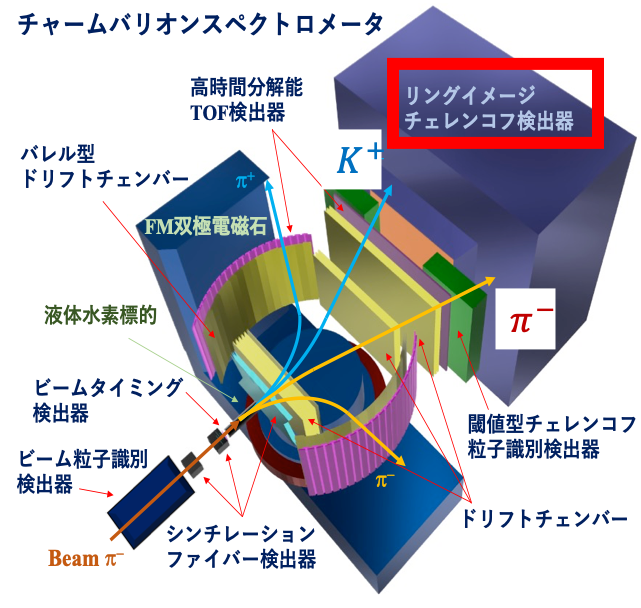
\includegraphics[clip, scale=0.8]{E50setup.png}
    \caption{E50実験のセットアップ。図後方のものがリングイメージチェレンコフ(RICH)検出器} 
    \label{fig:E50setup} 
  \end{center}
\end{figure}

$D^{*-}$の一連の崩壊から生じる$K^+, \pi^-$を2$\sim$16 GeV/{\sl c}の広い運動量領域で粒子識別を行う必要がある。そこで用いられるPID検出器が図\ref{fig:E50setup}後方のリングイメージチェレンコフ検出器である。

\section{測定原理}
 荷電粒子が物質中を通過する際にその速度が物質中の光速より早い場合、すなわち次式のような条件を満たす時、円錐状に光が発生する。
\begin{equation}
v > \frac{c}{n} \Leftrightarrow \beta > \frac{1}{n} 
\end{equation}
発生するチェレンコフ光と荷電粒子の進行方向がなす角をチェレンコフ角$\theta_c$と呼び、チェレンコフ角と荷電粒子の速度、物質の屈折率の関係は次式で表される。
\begin{equation}
\cos \theta_c = \frac{1}{n\beta}
\end{equation}
\begin{figure}[h]
  \begin{center} 
    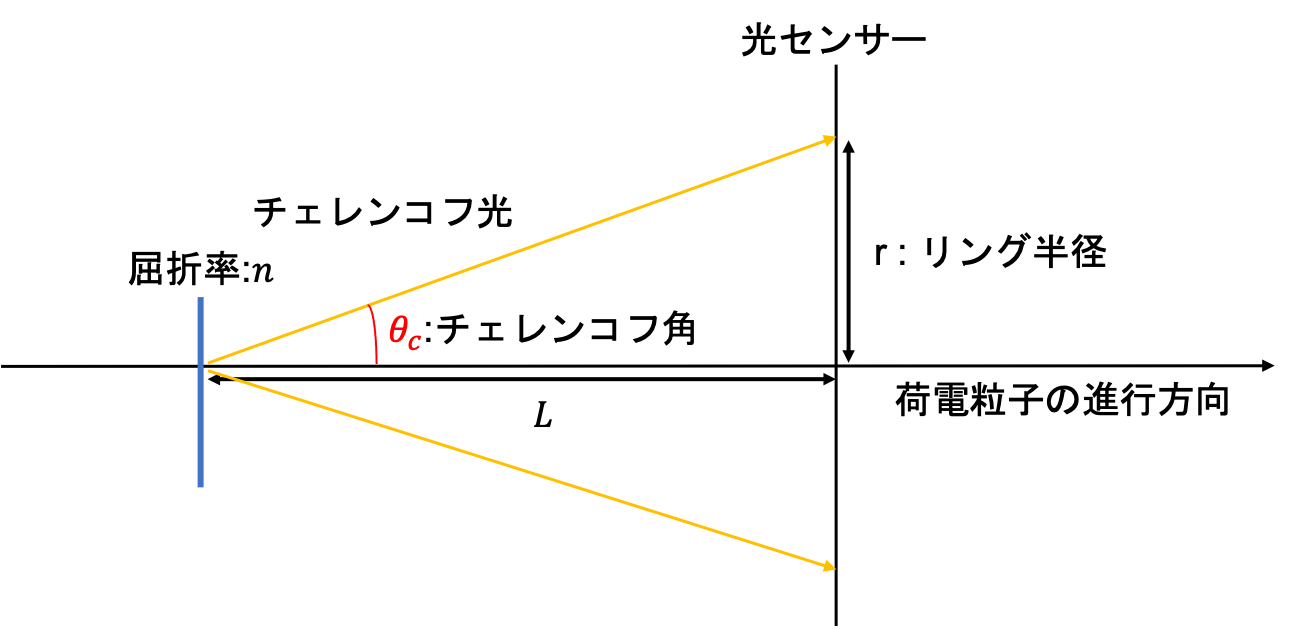
\includegraphics[clip, scale=0.5]{cherenkov.png}
    \caption{チェレンコフ光が発生する様子} 
    \label{fig:cherenkov} 
  \end{center}
\end{figure}

リングイメージチェレンコフ検出器では測定したリングイメージの半径と、輻射体から光センサーまでの距離$L$を用いて次の式からチェレンコフ角を算出する。
\begin{equation}
\tan \theta_c = \frac{r}{L} \Leftrightarrow \theta_c = \arctan \left(\frac{r}{L}\right)
\end{equation}
このチェレンコフ角を用いて式(1.4)より、粒子の速度を求めることで粒子識別を行う。
\begin{figure}[htbp]
  \begin{center}
    \begin{tabular}{c}

      % 1
      \begin{minipage}{0.33\hsize}
        \begin{center}
          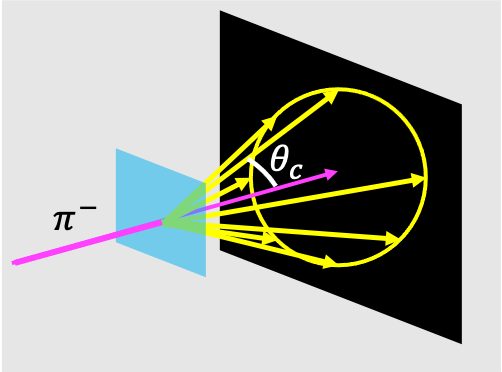
\includegraphics[clip, scale=0.6]{pion.png}
          \hspace{1.6cm}
        \end{center}
      \end{minipage}

      % 2
      \begin{minipage}{0.33\hsize}
        \begin{center}
          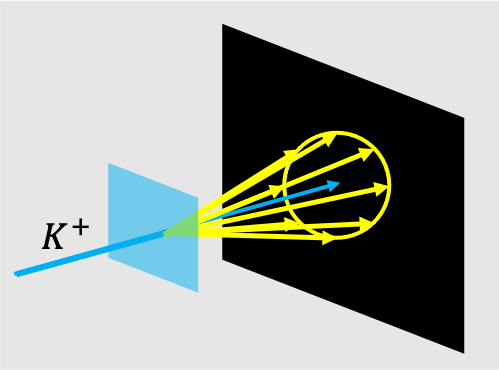
\includegraphics[clip, scale=0.6]{kaon.png}
          \hspace{1.6cm}
        \end{center}
      \end{minipage}

    \end{tabular}
    \caption{$\pi^-とK^+によるチェレンコフ光$}
    \label{fig:piKcherenkov}
  \end{center}
\end{figure}

\section{研究目的}
\subsection{先行研究によるRICH検出器実機の構成と要求性能}
 先行研究での実機の構成として、エアロゲル(n=1.04)と$\rm{C_4F_{10}}$ガス(n=1.0037)の2種類の輻射体を用いて、広い運動量領域においてチェレンコフ光を放出させる。このチェレンコフ光を球面鏡で反射させ、光センサー上で収束させることでリングイメージを観測する。

\begin{figure}[htbp]
  \begin{center} 
    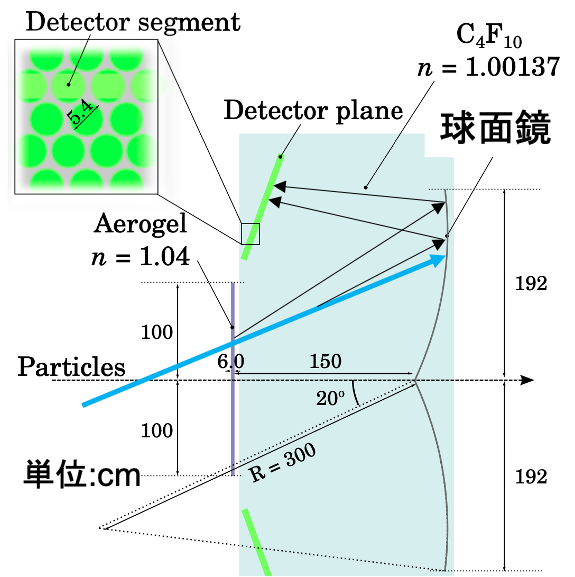
\includegraphics[clip, scale=0.8]{RICH.png}
    \caption{実機のデザイン(先行研究より)} 
    \label{fig:RICH} 
  \end{center}
\end{figure}
 実機の要求性能は次のようになっている。目標とする粒子識別性能99\%に要求される角度分解能は$\Delta\theta_c < 10 \rm{mrad}$であり、角度分解能は以下の要素に影響される。
\begin{enumerate}
  \item セグメントサイズの大きさによる位置分解能
  \item 色収差、輻射体の厚さによる分散、検出面での収束等の収差などの影響
  \item ビームの角度分解能
\end{enumerate}
このうち、収差などの影響の内訳は詳細にわかっていないため、球面鏡と光センサーとしてMPPCを用いた小型のテスト機を用いて収差の内訳について調査を行なった。
\subsection{Multi Pixel Photon Counter}
 今回のテスト実験で用いた光センサーであるMulti Pixel Photon Counter、MPPCは安価である、磁場に強いといった利点がある。一方で熱電子が増幅され、1光電子が常にノイズとして出ており、暗電流が大きいという特徴がある。その計数率は100~300kHzでありRICH検出器では1光電子を捉えるため、その影響についても併せて調査しシミュレーションによる再現を行なった。また電圧によってゲインと検出効率が変わるといった特徴もあり、以降ではMPPCの動作電圧$V_{operation}$から、信号が出始める電圧$V_{breakdown}\sim51V$を引いた$V_{over voltage}$という表記を用いる。
\chapter{実験のセットアップ}
  2020年12月にSPring-8のLEPSビームラインにて実験を行なった。0.95 GeV/$c$の電子・陽電子をビームとして用い、空気を輻射体とした。暗箱内にはビーム軸に対してチェレンコフ光が$15^\circ$の角度で反射するように球面鏡を配置し、MPPC上に収束させた。暗箱外側の先端と後部にはトリガーカウンターとして10mm角のプラスチックシンチレーターをそれぞれビーム軸上に配置した。
 
 \begin{figure}[htbp]
  \begin{center} 
    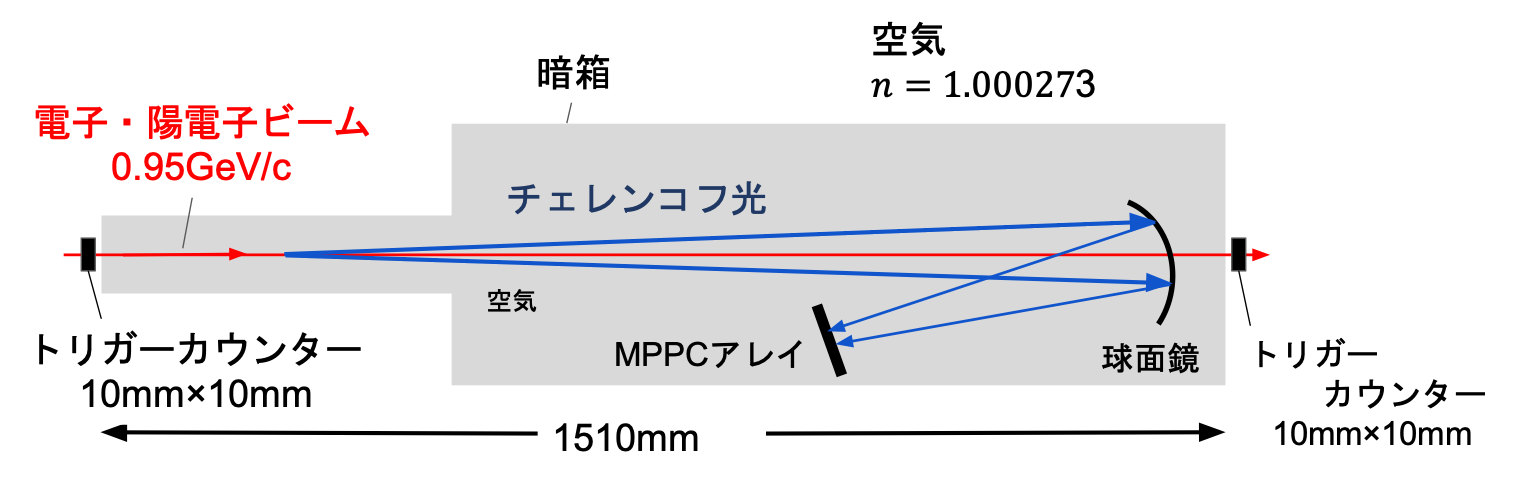
\includegraphics[clip, scale=0.6]{setup.png}
    \caption{実験のセットアップ}
    \label{fig:setup} 
  \end{center}
\end{figure}
MPPCは$8\times8$の2次元アレイ、64セグメントのもの使用し、1セグメントの大きさは3.2mm角である。動作電圧は54~57.5Vまで0.5V刻みで測定を行なった。読み出しにはNIM-EASIROC moduleを使用し、TDC情報を取得した。使用した球面鏡は直径が150mm、曲率半径は660mm、焦点距離はその半分の330mmである。

\begin{figure}[htbp]
  \begin{center}
    \begin{tabular}{c}

      % 1
      \begin{minipage}{0.33\hsize}
        \begin{center}
          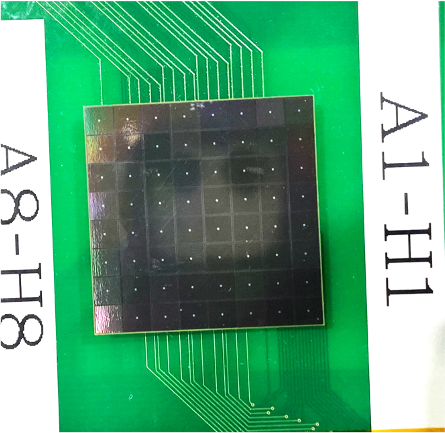
\includegraphics[clip, scale=0.6]{MPPC.png}
          \hspace{1.6cm} [1] MPPC
        \end{center}
      \end{minipage}

      % 2
      \begin{minipage}{0.33\hsize}
        \begin{center}
          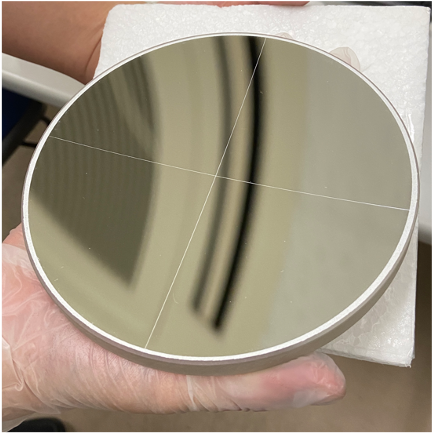
\includegraphics[clip, scale=0.6]{mirror.png}
          \hspace{1.6cm} [2] 球面鏡
        \end{center}
      \end{minipage}

    \end{tabular}
    \caption{使用したMPPCと球面鏡}
    \label{fig:MPPC'N'mirror}
  \end{center}
\end{figure}


\chapter{解析}
\section{TDC}
 TDCを取得するための閾値は動作電圧が最も低い$V_{ov}=3.0V$の時の1p.e.にかけた。取得したTDCのヒストグラムが次の図である。
 \begin{figure}[htbp]
  \begin{center} 
    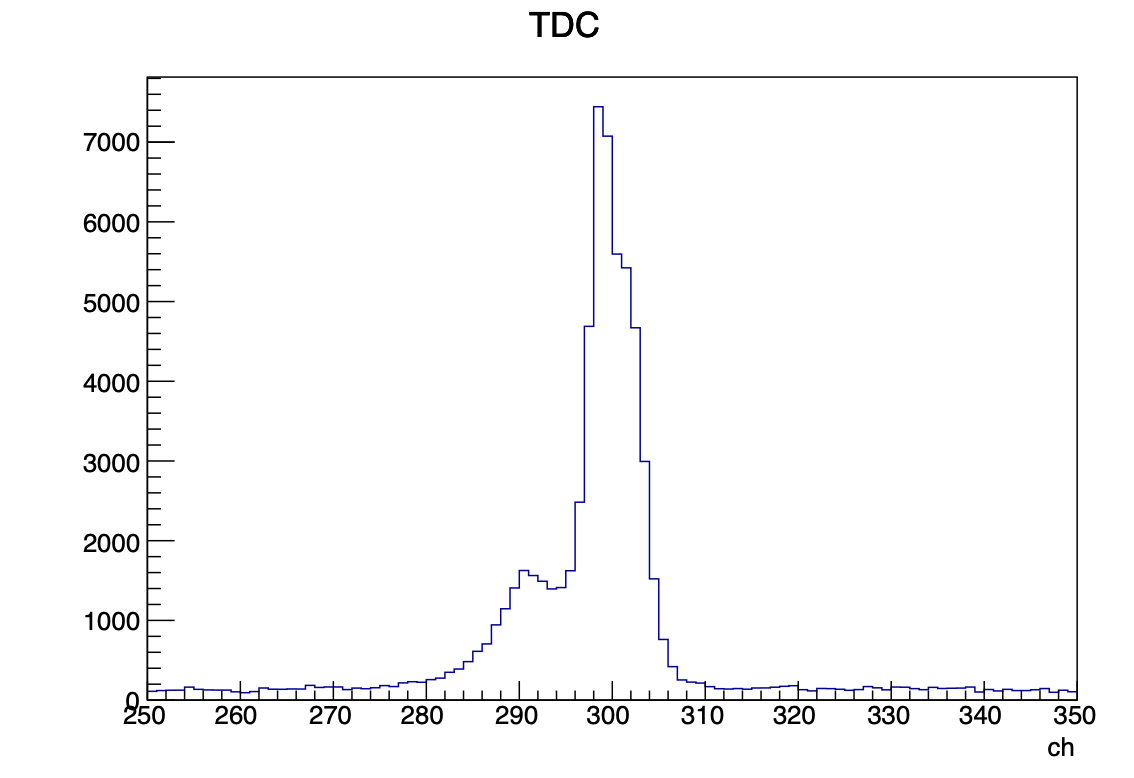
\includegraphics[clip, scale=0.3]{tdc.png}
    \caption{得られたTDCのヒストグラム。全てのチャンネルを足し合わせている。}
    \label{fig:tdc} 
  \end{center}
\end{figure}

\section{hit数}

\section{リングイメージの中心}
\subsection{決定方法1}
ここにはリング中心の求め方の一つ目を書く
\subsection{決定方法2}
ここにはリング中心の求め方の二つ目を書く

\section{リング半径・チェレンコフ角・角度分解能}

\chapter{結果}
\section{チェレンコフ角・角度分解能}

\section{理論値との比較}

\section{角度分解能の内訳}

\section{収差などによる角度分解能}

\section{暗電流の角度分解能への寄与}

\chapter{まとめ}
\end{document}  